\subsection{Methods}
The aim of this section is again to solve the environment of the Cartpole from the gym library. However, we will not use the 
observation space described in the previous section. We will instead use the cartpole displayed in a screen.
This task is far from easy, since the agent now have to infer the previous observation space from images. We first
decrease the size of the observation space, which is a $600\times400$ RGB image, as follows:
\begin{itemize}
    \item We transform the image in grayscale, passing from $3$ channels to $1$;
    \item We crop the image such that we have a small amount of empty screen, while still leaving to the cart the possibility
        of moving and being observed. In particular, we crop $150$ pixels from the bottom, $80$ from the top, $200$ from the left
        and $200$ from the right.
\end{itemize}
We so end up with a $200\times170$ grayscale image, as shown in Figure \ref{fig:image}. Still, we do not have any means of understanding
information about the velocity from a single image. We so concatenate $4$ subsequent images as input of the network. 

Since we fed images to the agent, in this case we decided to use a convolutional neural network, which architecture is presented in Figure
\ref{fig:conv}.
\begin{figure}[h]
    \centering
    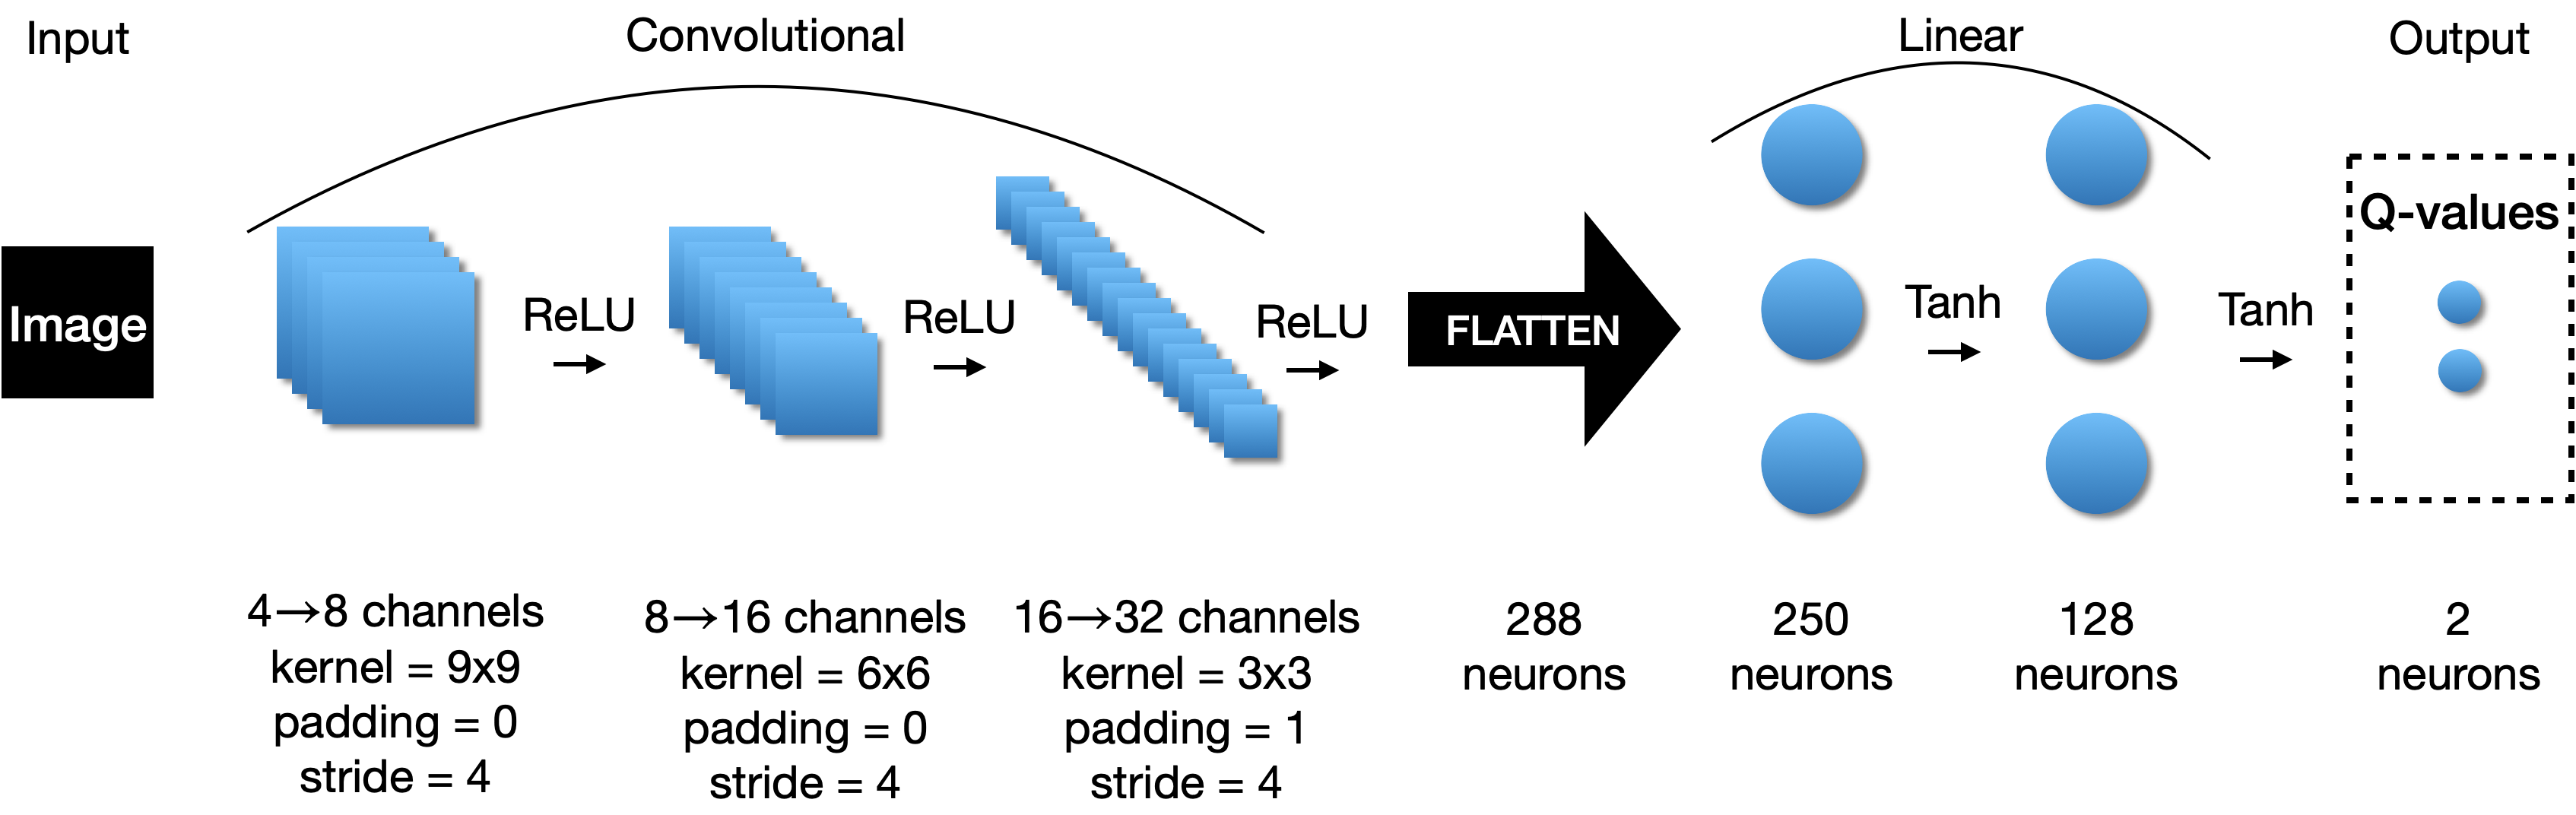
\includegraphics[width=0.7\textwidth]{Images/conv.png}
    \caption{Architecture of the convolutional neural network used as agent.}
    \label{fig:conv}
\end{figure}
It is important to notice that in the network we make plenty of use of the stride, which reduces the size of the image.

The firsts attempts were so difficult and low-performing that we thought of a trick to implement, divided into three main points:
\begin{itemize}
    \item Run the normal training, as in the previous section, but using the new observation space. Store the couples $[obs, st]$, where 
        $obs$ is given by the $4$ subsequent images defined above and $st$ is the state defined in Section \ref{sec:cart};
    \item Train a supervised convolutional neural network to predict $st$ given the $obs$, with the same structure shown in Figure \ref{fig:conv}, but where 
        the output layer has $4$ neurons instead of $2$;
    \item Perform transfer learning, by freezing the weights of the supervised network and attach to it a network with the same structure of Figure \ref{fig:dqnet}, and run
        the training again.
\end{itemize} 
This approach is particularly challenging due to the size of the $obs$, which quickly filled the RAM. It is however an interesting idea, and so we decided to present it 
anyway. 


\subsection{Results}
We used the best hyperparameter set found in the previous Section. As we can see in Figure \ref{fig:bef_trick} the network is able to learn a strategy to improve 
its score, thanks to all the tricks defined above. However, it is not able to solve the environment. We so decided to try to implement the procedure described 
above, adding a supervised part. The results of such a procedure are shown in Figure \ref{fig:aft_trick}. As we can observe, the results are worse than in the previous 
case, even if there is a learning. These results can be due to various problems of this task, first of all the scarcity of training samples for the supervised part,
on the order of $10\,000$, and not iid. Since the supervised part was not predicting the correct state the additional network was not able to produce meaningful
q-values.

We finally try to apply the same trick as above, but without freezing the weights of the previously trained network. The outcome is shown in Figure \ref{fig:nofreeze}. 
The learning is very unstable, and even if we manage to reach peaks of $200$ it is not clear if the performances really improve, or it is just a fluctuation.